\chapter{异步编程}\label{ch20}

假设你正在编写一个聊天服务器。每个网络连接都有很多要解析的到来的包、要组装的发送的包、要管理的安全参数、要追踪的聊天组订阅等。同时为许多连接管理所有这些信息需要进行一些组织。

理想情况下,你可以简单地为每一个到来的连接启动一个单独的线程:
\begin{minted}{Rust}
    use std::{net, thread};

    let listener = net::TcpListener::bind(address)?;

    for socket_result in listener.incoming() {
        let socket = socket_result?;
        let groups = chat_group_table.clone();
        thread::spawn(|| {
            log_error(serve(socket, groups));
        });
    }
\end{minted}

这样对每一个连接都会创建一个新的线程运行\texttt{serve}函数,这个函数专门处理一个连接的需求。

这可以正常工作,直到一切都比计划的更加顺利很多,然后突然你就已经有了几万名用户。一个线程的栈增长到100KB或更多并不罕见,你可能不想就这样花费几GB的内存。要把任务分发到多个处理器上,线程是合适并且必须的,但它们的内存需求太大以至于我们通常需要一些补充的方式和线程一起使用,来减小资源占用。

你可以使用Rust的\emph{异步任务(asynchronous task)}来在单个线程或者线程池中交替执行很多独立的任务。异步任务类似于线程,但可以更快地创建、更高效地传递控制权、并且内存开销比线程少一个数量级。在单个程序中同时运行数十万个异步任务是完全可行的。当然,你的应用仍然可能被其他因素限制,例如网络带宽、数据库速度、计算、或者任务本身的内存需求,但使用异步任务的固有内存开销比使用线程的要小很多。

一般来讲,异步Rust代码看起来和普通的多线程代码非常相似,除了那些可能阻塞的操作,例如I/O或获取锁的处理有一点不同。特殊对待这些操作让Rust有更多的信息了解你的代码的行为,这为进一步优化提供了可能。上面代码的异步版本看起来像这样:
\begin{minted}{Rust}
    use async_std::{net, task};

    let listener = net::TcpListener::bind(address).await?;

    let mut new_connections = listener.incoming();
    while let Some(socket_result) = new_connections.next().await {
        let socket = socket_result?;
        let groups = chat_group_table.clone();
        task::spawn(async {
            log_error(serve(socket, groups).await);
        });
    }
\end{minted}

这里使用了\texttt{async\_std} crate的网络和任务模块,并在可能阻塞的调用后加上了\texttt{.await}。但整体的结构和基于线程的版本一样。

这一章的目标不止是帮你编写异步代码,还要向你展示它的工作细节,以便你可以预测它在你的应用中的表现,并了解它在哪些方面最有价值。

\begin{enumerate}
    \item 为了展示异步编程的机制,我们列出了涵盖所有核心概念的最小语言功能集:future、异步函数、\texttt{await}表达式、task、\texttt{block\_on}和\texttt{spawn\_local} executor。
    \item 然后我们会展示异步块和\texttt{spawn} executor。它们是完成真实工作的最基础的部分,但从概念上讲,它们只是我们刚才提到过的功能的变体。在这个过程中,我们会指出一些你可能会遇到的异步编程特有的问题并解释如何处理它们。
    \item 为了展示所有功能的协调工作,我们会展示一个聊天服务器和客户端的完整代码,上面的代码片段就是其中一部分。
    \item 为了演示原语future和executor如何工作,我们会展示\texttt{spawn\_blocking}和\texttt{block\_on}的简单实现。
    \item 最后,我们介绍了异步接口中经常出现的\texttt{Pin}类型,它被用来确保异步函数和块future被安全地使用。
\end{enumerate}

\section{从同步到异步}

考虑当你调用下面的(不是异步的)函数时会发生什么:
\begin{minted}{Rust}
    use std::io::prelude::*;
    use std::net;

    fn cheapo_request(host: &str, port: u16, path: &str)
                          -> std::io::Result<String>
    {
        let mut socket = net::TcpStream::connect((host, port))?;

        let request = format!("GET {} HTTP/1.1\r\nHost: {}\r\n\r\n", path, host);
        socket.write_all(request.as_bytes())?;
        socket.shutdown(net::Shutdown::Write)?;

        let mut response = String::new();
        socket.read_to_string(&mut response)?;

        Ok(response)
    }
\end{minted}

这会打开一个到web服务器的TCP连接,以过时的协议向它发送一个简单的HTTP请求,\footnote{如果你真的需要一个HTTP客户端,考虑使用一些非常优秀的crate例如\texttt{surf}或\texttt{reqwest},它们会正确并且异步地完成任务。这个客户端基本只是设法获得HTTPS重定向。}然后读取响应。\autoref{f20-1}展示了这个函数的执行过程随时间的变化。

\begin{figure}[htbp]
    \centering
    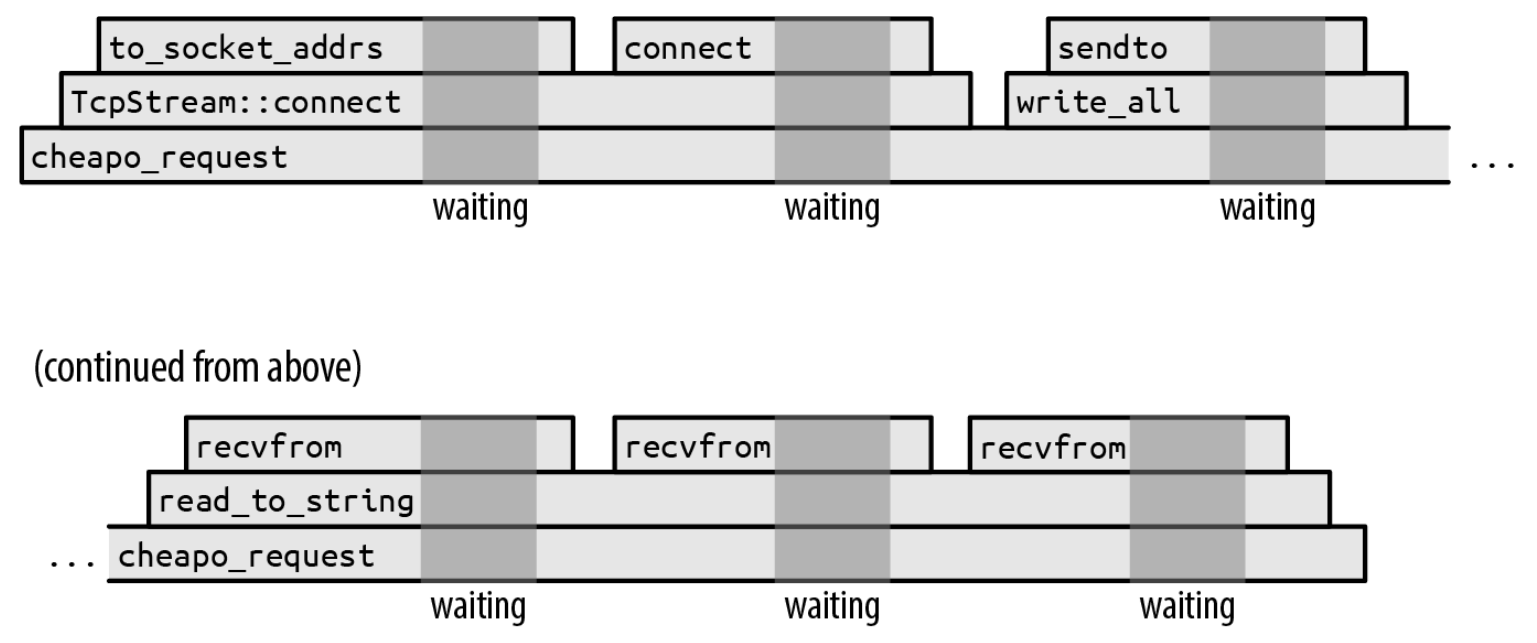
\includegraphics[width=0.8\textwidth]{../img/f20-1.png}
    \caption{一个同步HTTP请求的过程(深颜色的区域标识等待操作系统)}
    \label{f20-1}
\end{figure}

图中展示了从左到右随着时间的推移,函数的调用栈的变化。每一个函数调用都是一个方块,位于它的调用者上面。显然,\texttt{cheapo\_request}函数贯穿整个执行过程。它调用了Rust标准库里的函数例如\texttt{TcpStream::connect}和\texttt{TcpStream}的\texttt{write\_all}和\texttt{read\_to\_string}实现。这些对其他函数的调用依次进行,但最终程序会进行\emph{系统调用},请求操作系统完成真正的工作,例如打开TCP连接,或者读写一些数据。

深灰色的区域表示程序正在等待操作系统完成系统调用。我们并没有按比例绘制这些时间。因为加入我们按比例绘制,整个图都将是深灰色:在实践中,这个函数把几乎所有时间都用在等待操作系统上。上面代码的执行时间将是系统调用之间的窄条。

当函数等待系统调用返回时,它所在的线程会阻塞住:它不能做任何事,直到系统调用结束。一个线程的栈达到几百或几千字节并不罕见,因此如果这是一个更大的系统的一部分,并且有很多线程做类似的任务,锁住这些线程的资源但除了等待什么也不做的代价是非常昂贵的。

为了解决这个问题,一个线程需要能在等待系统调用完成的同时去执行其他的任务。但如何实现这一点并不明显。例如,我们用来从套接字读取响应的函数的签名是:
\begin{minted}{Rust}
    fn read_to_string(&mut self, buf: &mut String) -> std::io::Result<usize>;
\end{minted}

它的类型表明了:这个函数直到工作完成或者出错时才会返回。这个函数是\emph{同步的}:当操作完成时调用者才恢复。如果我们想在操作系统进行工作的同时用我们的线程去做别的任务,那么我们需要一个新的提供这个函数的\emph{异步}版本的I/O库。

\subsection{\texttt{Future}}
Rust支持异步操作的方法是引入一个trait:\texttt{std::future::Future}:
\begin{minted}{Rust}
    trait Future {
        type Output;
        // 现在,把`Pin<&mut Self>`看作`&mut Self`就好了。
        fn poll(self: Pin<&mut Self>, cx: &mut Context<'_>) -> Poll<Self::Output>;
    }

    enum Poll<T> {
        Ready(T),
        Pending,
    }
\end{minted}

一个\texttt{Future}代表一个可以测试是否完成的操作。一个future的\texttt{poll}方法从来不会等待操作完成:它总是立即返回。如果操作完成了,\texttt{poll}会返回\texttt{Poll::Ready(output)},其中\texttt{output}是最后的结果。否则,它会返回\texttt{Pending}。当且仅当future值得再次poll时,它会通过调用一个\emph{waker}来通知我们,这是一个由\texttt{Context}提供的回调函数。我们称之为异步编程的“piñata 模型” :你唯一能对future做的就是使用\texttt{poll}敲打它,直到有一个值掉出来。

所有现代的操作系统都包含一些系统调用的变体,我们可以用它们来实现这种poll接口。例如在Unix和Windows上,如果你把网络套接字设置为非阻塞模式,那么如果它们正在阻塞时进行read和write会返回错误,你必须稍后再试。

因此\texttt{read\_to\_string}的一个异步版本的签名大概是这样:
\begin{minted}{Rust}
    fn read_to_string(&mut self, buf: &mut String)
        -> impl Future<Output = Result<usize>;
\end{minted}

除了返回类型之外,这和我们之前展示的签名一样:异步的版本返回\emph{一个\texttt{Result<usize>}的future}。你需要poll这个future,直到从它得到一个\texttt{Ready(result)}。每次它被poll时,都会尽可能地继续读取。最后的\texttt{result}给你成功的值或者错误的值,就像普通的I/O操作一样。这是通常的模式:异步版本的任何函数和同步版本的函数获取相同的参数,但返回类型有一个\texttt{Future}包装。

调用这个版本的\texttt{read\_to\_string}并不会真的读取任何内容;它所有的任务就是构造并返回一个future,这个future会在被poll时进行真正的工作。这个future必须包含处理请求所需的所有信息。例如,这个\texttt{read\_to\_string}返回的future必须记住调用它的输入流,和它需要写入数据的\texttt{String}。事实上,因为这个future持有了\texttt{self}和\texttt{buf}的引用,因此这个\texttt{read\_to\_string}的真正的签名必须是:
\begin{minted}{Rust}
    fn read_to_string<'a>(&'a mut self, buf: &'a mut String)
        -> impl Future<Output = Result<usize>> + 'a;
\end{minted}

这个附加的生命周期指示了返回的future和它借用的\texttt{self}和\texttt{buf}的生命周期一样长。

\texttt{async-std} crate提供了\texttt{std}的所有I/O设施的异步版本,包括一个有\texttt{read\_to\_string}方法的异步\texttt{Read} trait。\texttt{async-std}密切地遵循了\texttt{std}的设计,尽可能地在自己的接口中重用\texttt{std}的类型,因此这两个世界中的错误、结果、网络地址、和其他大多数相关的数据都是兼容的。熟悉\texttt{std}有助于使用\texttt{async-std},反之亦然。

\texttt{Future} trait的一个规则是,一旦一个future返回了\texttt{Poll::Ready},它会假设它决不会再次被poll。一些future在自己被overpoll时简单地永远返回\texttt{Poll::Pending};其它的可能panic或者挂起。(它们绝不能违反内存或线程安全性,或者导致未定义行为)\texttt{Future} trait的\texttt{fuse}适配器将任何future转换成overpoll时永远返回\texttt{Poll::Pending}。但通常消费future的方法都遵循这个规则,因此\texttt{fuse}通常不是必须的。

如果poll听起来效率底下,请不必担心。Rust的异步架构是精心设计的,所以只要你的基本I/O函数例如\texttt{read\_to\_string}是正确实现的,那么你只会在值的时poll一个future。每一次\texttt{poll}被调用时,某个东西应该返回\texttt{Ready},或者至少向目标前进一步。我们将在“\nameref{WhenPoll}”中解释这是如何工作的。

但使用future看起来有一个挑战:当你poll时,如果你得到了\texttt{Poll::Pending}那你应该怎么做?你将不得不四处寻找这个线程暂时可以做的其他工作,并记住一段时间之后返回到这个future,然后再次poll。你的整个系统将因为持续追踪谁正在pending和当它们完成时应该做什么而变得杂乱无章。我们的\texttt{cheapo\_request}函数的简洁性会被破坏。

好消息是:它并不是这样的!

\subsection{\texttt{async}函数和\texttt{await}表达式}

\section{原语future和executor:何时一个future值得再次poll}\label{WhenPoll}